\documentclass[1p]{elsarticle_modified}
%\bibliographystyle{elsarticle-num}

%\usepackage[colorlinks]{hyperref}
%\usepackage{abbrmath_seonhwa} %\Abb, \Ascr, \Acal ,\Abf, \Afrak
\usepackage{amsfonts}
\usepackage{amssymb}
\usepackage{amsmath}
\usepackage{amsthm}
\usepackage{scalefnt}
\usepackage{amsbsy}
\usepackage{kotex}
\usepackage{caption}
\usepackage{subfig}
\usepackage{color}
\usepackage{graphicx}
\usepackage{xcolor} %% white, black, red, green, blue, cyan, magenta, yellow
\usepackage{float}
\usepackage{setspace}
\usepackage{hyperref}

\usepackage{tikz}
\usetikzlibrary{arrows}

\usepackage{multirow}
\usepackage{array} % fixed length table
\usepackage{hhline}

%%%%%%%%%%%%%%%%%%%%%
\makeatletter
\renewcommand*\env@matrix[1][\arraystretch]{%
	\edef\arraystretch{#1}%
	\hskip -\arraycolsep
	\let\@ifnextchar\new@ifnextchar
	\array{*\c@MaxMatrixCols c}}
\makeatother %https://tex.stackexchange.com/questions/14071/how-can-i-increase-the-line-spacing-in-a-matrix
%%%%%%%%%%%%%%%

\usepackage[normalem]{ulem}

\newcommand{\msout}[1]{\ifmmode\text{\sout{\ensuremath{#1}}}\else\sout{#1}\fi}
%SOURCE: \msout is \stkout macro in https://tex.stackexchange.com/questions/20609/strikeout-in-math-mode

\newcommand{\cancel}[1]{
	\ifmmode
	{\color{red}\msout{#1}}
	\else
	{\color{red}\sout{#1}}
	\fi
}

\newcommand{\add}[1]{
	{\color{blue}\uwave{#1}}
}

\newcommand{\replace}[2]{
	\ifmmode
	{\color{red}\msout{#1}}{\color{blue}\uwave{#2}}
	\else
	{\color{red}\sout{#1}}{\color{blue}\uwave{#2}}
	\fi
}

\newcommand{\Sol}{\mathcal{S}} %segment
\newcommand{\D}{D} %diagram
\newcommand{\A}{\mathcal{A}} %arc


%%%%%%%%%%%%%%%%%%%%%%%%%%%%%5 test

\def\sl{\operatorname{\textup{SL}}(2,\Cbb)}
\def\psl{\operatorname{\textup{PSL}}(2,\Cbb)}
\def\quan{\mkern 1mu \triangleright \mkern 1mu}

\theoremstyle{definition}
\newtheorem{thm}{Theorem}[section]
\newtheorem{prop}[thm]{Proposition}
\newtheorem{lem}[thm]{Lemma}
\newtheorem{ques}[thm]{Question}
\newtheorem{cor}[thm]{Corollary}
\newtheorem{defn}[thm]{Definition}
\newtheorem{exam}[thm]{Example}
\newtheorem{rmk}[thm]{Remark}
\newtheorem{alg}[thm]{Algorithm}

\newcommand{\I}{\sqrt{-1}}
\begin{document}

%\begin{frontmatter}
%
%\title{Boundary parabolic representations of knots up to 8 crossings}
%
%%% Group authors per affiliation:
%\author{Yunhi Cho} 
%\address{Department of Mathematics, University of Seoul, Seoul, Korea}
%\ead{yhcho@uos.ac.kr}
%
%
%\author{Seonhwa Kim} %\fnref{s_kim}}
%\address{Center for Geometry and Physics, Institute for Basic Science, Pohang, 37673, Korea}
%\ead{ryeona17@ibs.re.kr}
%
%\author{Hyuk Kim}
%\address{Department of Mathematical Sciences, Seoul National University, Seoul 08826, Korea}
%\ead{hyukkim@snu.ac.kr}
%
%\author{Seokbeom Yoon}
%\address{Department of Mathematical Sciences, Seoul National University, Seoul, 08826,  Korea}
%\ead{sbyoon15@snu.ac.kr}
%
%\begin{abstract}
%We find all boundary parabolic representation of knots up to 8 crossings.
%
%\end{abstract}
%\begin{keyword}
%    \MSC[2010] 57M25 
%\end{keyword}
%
%\end{frontmatter}

%\linenumbers
%\tableofcontents
%
\newcommand\colored[1]{\textcolor{white}{\rule[-0.35ex]{0.8em}{1.4ex}}\kern-0.8em\color{red} #1}%
%\newcommand\colored[1]{\textcolor{white}{ #1}\kern-2.17ex	\textcolor{white}{ #1}\kern-1.81ex	\textcolor{white}{ #1}\kern-2.15ex\color{red}#1	}

{\Large $\underline{12a_{0619}~(K12a_{0619})}$}

\setlength{\tabcolsep}{10pt}
\renewcommand{\arraystretch}{1.6}
\vspace{1cm}\begin{tabular}{m{100pt}>{\centering\arraybackslash}m{274pt}}
\multirow{5}{120pt}{
	\centering
	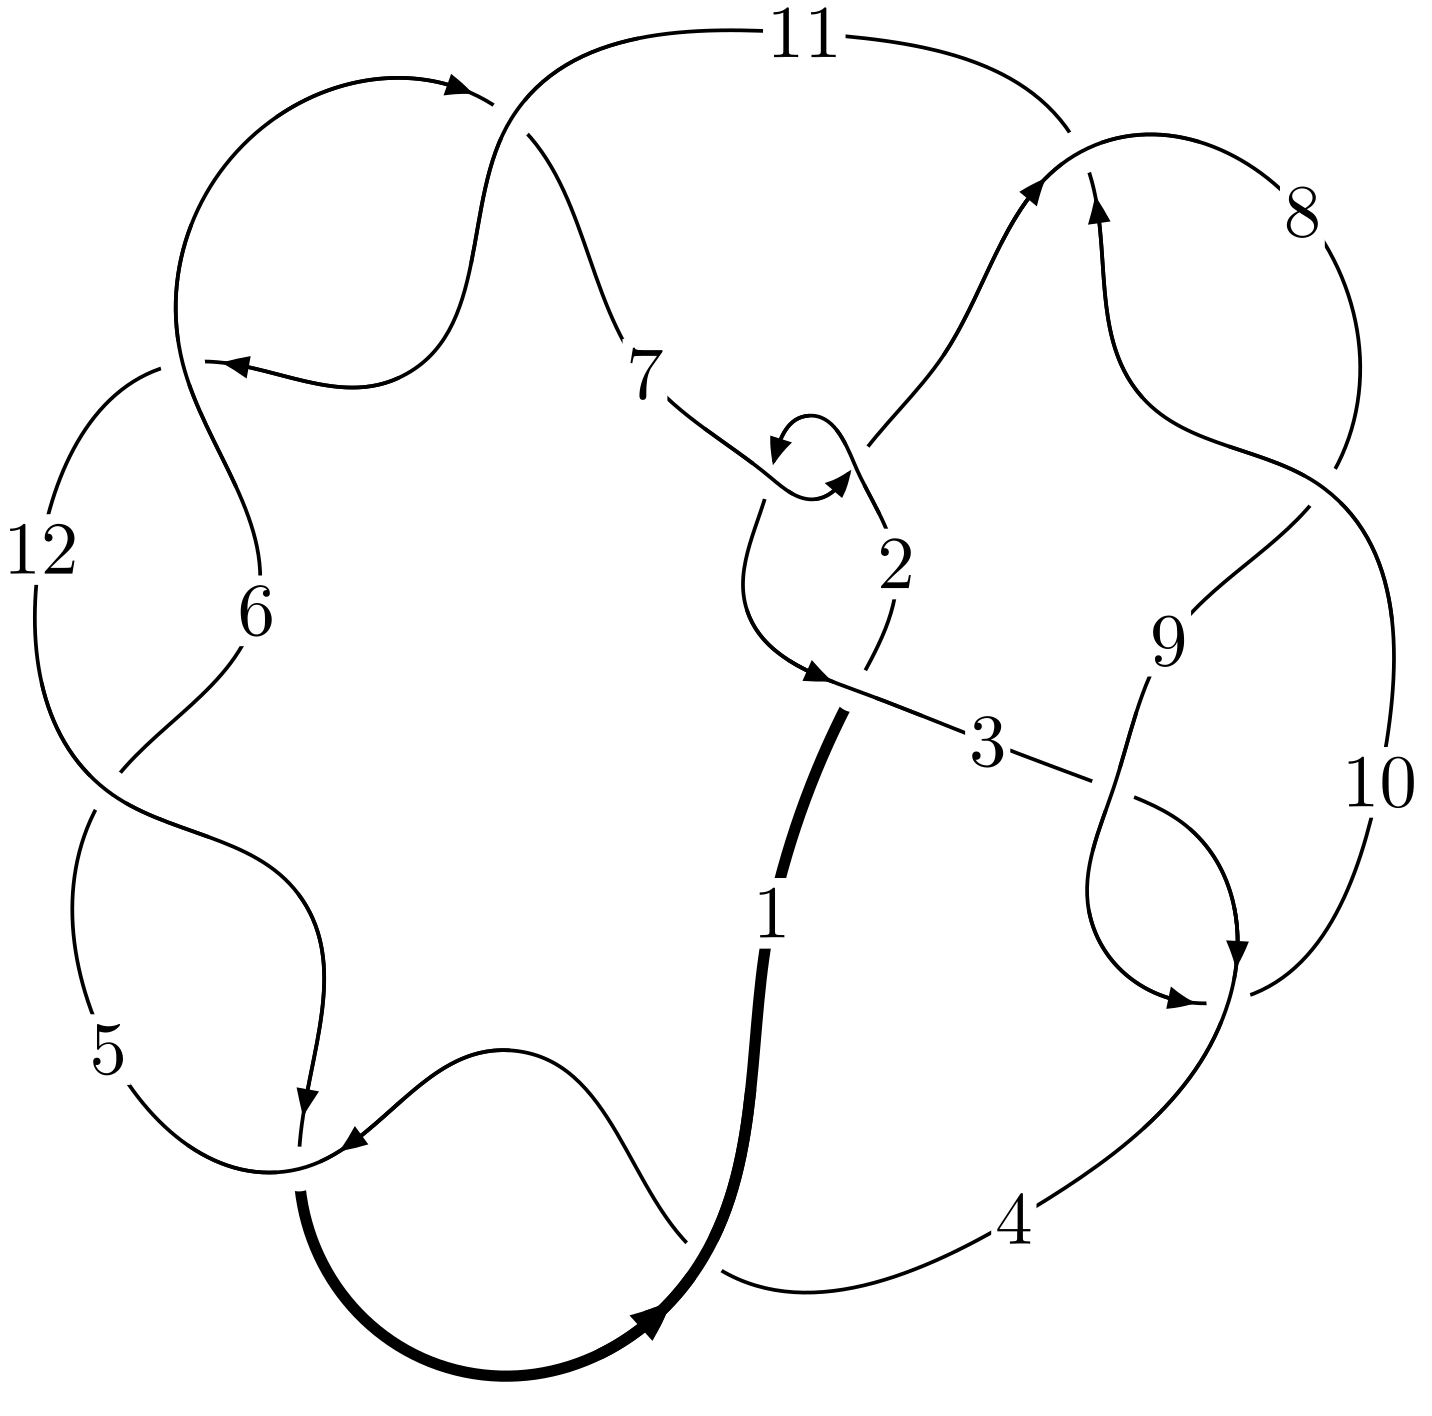
\includegraphics[width=112pt]{../../../GIT/diagram.site/Diagrams/png/1420_12a_0619.png}\\
\ \ \ A knot diagram\footnotemark}&
\allowdisplaybreaks
\textbf{Linearized knot diagam} \\
\cline{2-2}
 &
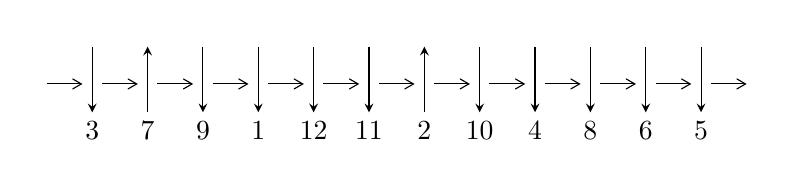
\begin{tikzpicture}[x=20pt, y=17pt]
	% nodes
	\node (C0) at (0, 0) {};
	\node (C1) at (1, 0) {};
	\node (C1U) at (1, +1) {};
	\node (C1D) at (1, -1) {3};

	\node (C2) at (2, 0) {};
	\node (C2U) at (2, +1) {};
	\node (C2D) at (2, -1) {7};

	\node (C3) at (3, 0) {};
	\node (C3U) at (3, +1) {};
	\node (C3D) at (3, -1) {9};

	\node (C4) at (4, 0) {};
	\node (C4U) at (4, +1) {};
	\node (C4D) at (4, -1) {1};

	\node (C5) at (5, 0) {};
	\node (C5U) at (5, +1) {};
	\node (C5D) at (5, -1) {12};

	\node (C6) at (6, 0) {};
	\node (C6U) at (6, +1) {};
	\node (C6D) at (6, -1) {11};

	\node (C7) at (7, 0) {};
	\node (C7U) at (7, +1) {};
	\node (C7D) at (7, -1) {2};

	\node (C8) at (8, 0) {};
	\node (C8U) at (8, +1) {};
	\node (C8D) at (8, -1) {10};

	\node (C9) at (9, 0) {};
	\node (C9U) at (9, +1) {};
	\node (C9D) at (9, -1) {4};

	\node (C10) at (10, 0) {};
	\node (C10U) at (10, +1) {};
	\node (C10D) at (10, -1) {8};

	\node (C11) at (11, 0) {};
	\node (C11U) at (11, +1) {};
	\node (C11D) at (11, -1) {6};

	\node (C12) at (12, 0) {};
	\node (C12U) at (12, +1) {};
	\node (C12D) at (12, -1) {5};
	\node (C13) at (13, 0) {};

	% arrows
	\draw[->,>={angle 60}]
	(C0) edge (C1) (C1) edge (C2) (C2) edge (C3) (C3) edge (C4) (C4) edge (C5) (C5) edge (C6) (C6) edge (C7) (C7) edge (C8) (C8) edge (C9) (C9) edge (C10) (C10) edge (C11) (C11) edge (C12) (C12) edge (C13) ;	\draw[->,>=stealth]
	(C1U) edge (C1D) (C2D) edge (C2U) (C3U) edge (C3D) (C4U) edge (C4D) (C5U) edge (C5D) (C6U) edge (C6D) (C7D) edge (C7U) (C8U) edge (C8D) (C9U) edge (C9D) (C10U) edge (C10D) (C11U) edge (C11D) (C12U) edge (C12D) ;
	\end{tikzpicture} \\
\hhline{~~} \\& 
\textbf{Solving Sequence} \\ \cline{2-2} 
 &
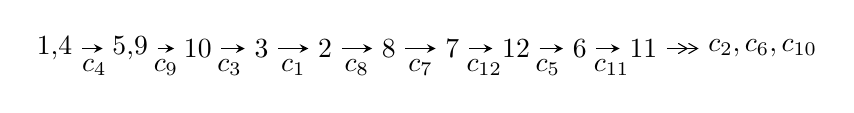
\begin{tikzpicture}[x=23pt, y=7pt]
	% node
	\node (A0) at (-1/8, 0) {1,4};
	\node (A1) at (17/16, 0) {5,9};
	\node (A2) at (17/8, 0) {10};
	\node (A3) at (25/8, 0) {3};
	\node (A4) at (33/8, 0) {2};
	\node (A5) at (41/8, 0) {8};
	\node (A6) at (49/8, 0) {7};
	\node (A7) at (57/8, 0) {12};
	\node (A8) at (65/8, 0) {6};
	\node (A9) at (73/8, 0) {11};
	\node (C1) at (1/2, -1) {$c_{4}$};
	\node (C2) at (13/8, -1) {$c_{9}$};
	\node (C3) at (21/8, -1) {$c_{3}$};
	\node (C4) at (29/8, -1) {$c_{1}$};
	\node (C5) at (37/8, -1) {$c_{8}$};
	\node (C6) at (45/8, -1) {$c_{7}$};
	\node (C7) at (53/8, -1) {$c_{12}$};
	\node (C8) at (61/8, -1) {$c_{5}$};
	\node (C9) at (69/8, -1) {$c_{11}$};
	\node (A10) at (11, 0) {$c_{2},c_{6},c_{10}$};

	% edge
	\draw[->,>=stealth]	
	(A0) edge (A1) (A1) edge (A2) (A2) edge (A3) (A3) edge (A4) (A4) edge (A5) (A5) edge (A6) (A6) edge (A7) (A7) edge (A8) (A8) edge (A9) ;
	\draw[->>,>={angle 60}]	
	(A9) edge (A10);
\end{tikzpicture} \\ 

\end{tabular} \\

\footnotetext{
The image of knot diagram is generated by the software ``\textbf{Draw programme}" developed by Andrew Bartholomew(\url{http://www.layer8.co.uk/maths/draw/index.htm\#Running-draw}), where we modified some parts for our purpose(\url{https://github.com/CATsTAILs/LinksPainter}).
}\phantom \\ \newline 
\centering \textbf{Ideals for irreducible components\footnotemark of $X_{\text{par}}$} 
 
\begin{align*}
I^u_{1}&=\langle 
-1.85075\times10^{26} u^{54}-1.82177\times10^{26} u^{53}+\cdots+5.53593\times10^{26} b+1.34110\times10^{27},\\
\phantom{I^u_{1}}&\phantom{= \langle  }2.89480\times10^{27} u^{54}+2.68152\times10^{27} u^{53}+\cdots+5.53593\times10^{26} a-2.16054\times10^{28},\;u^{55}+u^{54}+\cdots-12 u-1\rangle \\
I^u_{2}&=\langle 
- u^3 a+u^2 a+5 u^3-4 a u+5 b- a+10 u,\;- u^3 a- u^2 a+2 u^3+a^2-2 a u+u^2-2 a+6 u+2,\;u^4+3 u^2+1\rangle \\
\\
\end{align*}
\raggedright * 2 irreducible components of $\dim_{\mathbb{C}}=0$, with total 63 representations.\\
\footnotetext{All coefficients of polynomials are rational numbers. But the coefficients are sometimes approximated in decimal forms when there is not enough margin.}
\newpage
\renewcommand{\arraystretch}{1}
\centering \section*{I. $I^u_{1}= \langle -1.85\times10^{26} u^{54}-1.82\times10^{26} u^{53}+\cdots+5.54\times10^{26} b+1.34\times10^{27},\;2.89\times10^{27} u^{54}+2.68\times10^{27} u^{53}+\cdots+5.54\times10^{26} a-2.16\times10^{28},\;u^{55}+u^{54}+\cdots-12 u-1 \rangle$}
\flushleft \textbf{(i) Arc colorings}\\
\begin{tabular}{m{7pt} m{180pt} m{7pt} m{180pt} }
\flushright $a_{1}=$&$\begin{pmatrix}0\\u\end{pmatrix}$ \\
\flushright $a_{4}=$&$\begin{pmatrix}1\\0\end{pmatrix}$ \\
\flushright $a_{5}=$&$\begin{pmatrix}1\\u^2\end{pmatrix}$ \\
\flushright $a_{9}=$&$\begin{pmatrix}-5.22911 u^{54}-4.84385 u^{53}+\cdots+184.977 u+39.0276\\0.334317 u^{54}+0.329082 u^{53}+\cdots-18.1099 u-2.42254\end{pmatrix}$ \\
\flushright $a_{10}=$&$\begin{pmatrix}-5.56342 u^{54}-5.17293 u^{53}+\cdots+203.087 u+41.4501\\0.334317 u^{54}+0.329082 u^{53}+\cdots-18.1099 u-2.42254\end{pmatrix}$ \\
\flushright $a_{3}=$&$\begin{pmatrix}2.01049 u^{54}+1.47507 u^{53}+\cdots-60.3680 u-18.1292\\-1.17670 u^{54}-0.737240 u^{53}+\cdots+28.3449 u+5.00114\end{pmatrix}$ \\
\flushright $a_{2}=$&$\begin{pmatrix}-3.21401 u^{54}-2.21018 u^{53}+\cdots+93.1627 u+24.4667\\1.00340 u^{54}+0.579236 u^{53}+\cdots-25.9928 u-4.57326\end{pmatrix}$ \\
\flushright $a_{8}=$&$\begin{pmatrix}-6.41607 u^{54}-5.63866 u^{53}+\cdots+226.145 u+38.8714\\-0.416211 u^{54}-0.438802 u^{53}+\cdots+21.9914 u+4.79282\end{pmatrix}$ \\
\flushright $a_{7}=$&$\begin{pmatrix}u^4+3 u^2+1\\u^6+4 u^4+3 u^2\end{pmatrix}$ \\
\flushright $a_{12}=$&$\begin{pmatrix}u\\u^3+u\end{pmatrix}$ \\
\flushright $a_{6}=$&$\begin{pmatrix}u^2+1\\u^4+2 u^2\end{pmatrix}$ \\
\flushright $a_{11}=$&$\begin{pmatrix}u^3+2 u\\u^5+3 u^3+u\end{pmatrix}$\\&\end{tabular}
\flushleft \textbf{(ii) Obstruction class $= -1$}\\~\\
\flushleft \textbf{(iii) Cusp Shapes $= \frac{1012232232711983767701675065}{276796444336859447752049744} u^{54}+\frac{676329581383746073717624245}{276796444336859447752049744} u^{53}+\cdots-\frac{6753618946943674742901539099}{69199111084214861938012436} u-\frac{9459757630078072988532524263}{276796444336859447752049744}$}\\~\\
\newpage\renewcommand{\arraystretch}{1}
\flushleft \textbf{(iv) u-Polynomials at the component}\newline \\
\begin{tabular}{m{50pt}|m{274pt}}
Crossings & \hspace{64pt}u-Polynomials at each crossing \\
\hline $$\begin{aligned}c_{1}\end{aligned}$$&$\begin{aligned}
&u^{55}+23 u^{54}+\cdots+88 u-16
\end{aligned}$\\
\hline $$\begin{aligned}c_{2},c_{7}\end{aligned}$$&$\begin{aligned}
&u^{55}+u^{54}+\cdots-8 u+4
\end{aligned}$\\
\hline $$\begin{aligned}c_{3},c_{9}\end{aligned}$$&$\begin{aligned}
&u^{55}+u^{54}+\cdots+6 u+5
\end{aligned}$\\
\hline $$\begin{aligned}c_{4},c_{5},c_{6}\\c_{11},c_{12}\end{aligned}$$&$\begin{aligned}
&u^{55}- u^{54}+\cdots-12 u+1
\end{aligned}$\\
\hline $$\begin{aligned}c_{8},c_{10}\end{aligned}$$&$\begin{aligned}
&u^{55}+17 u^{54}+\cdots+56 u+25
\end{aligned}$\\
\hline
\end{tabular}\\~\\
\newpage\renewcommand{\arraystretch}{1}
\flushleft \textbf{(v) Riley Polynomials at the component}\newline \\
\begin{tabular}{m{50pt}|m{274pt}}
Crossings & \hspace{64pt}Riley Polynomials at each crossing \\
\hline $$\begin{aligned}c_{1}\end{aligned}$$&$\begin{aligned}
&y^{55}+27 y^{54}+\cdots+50976 y-256
\end{aligned}$\\
\hline $$\begin{aligned}c_{2},c_{7}\end{aligned}$$&$\begin{aligned}
&y^{55}+23 y^{54}+\cdots+88 y-16
\end{aligned}$\\
\hline $$\begin{aligned}c_{3},c_{9}\end{aligned}$$&$\begin{aligned}
&y^{55}-17 y^{54}+\cdots+56 y-25
\end{aligned}$\\
\hline $$\begin{aligned}c_{4},c_{5},c_{6}\\c_{11},c_{12}\end{aligned}$$&$\begin{aligned}
&y^{55}+75 y^{54}+\cdots+84 y-1
\end{aligned}$\\
\hline $$\begin{aligned}c_{8},c_{10}\end{aligned}$$&$\begin{aligned}
&y^{55}+47 y^{54}+\cdots+41236 y-625
\end{aligned}$\\
\hline
\end{tabular}\\~\\
\newpage\flushleft \textbf{(vi) Complex Volumes and Cusp Shapes}
$$\begin{array}{c|c|c}  
\text{Solutions to }I^u_{1}& \I (\text{vol} + \sqrt{-1}CS) & \text{Cusp shape}\\
 \hline 
\begin{aligned}
u &= -0.242174 + 0.965422 I \\
a &= \phantom{-}1.84242 + 0.74241 I \\
b &= \phantom{-}1.088040 - 0.231202 I\end{aligned}
 & -0.05193 + 5.45928 I & \phantom{-0.000000 } 0 \\ \hline\begin{aligned}
u &= -0.242174 - 0.965422 I \\
a &= \phantom{-}1.84242 - 0.74241 I \\
b &= \phantom{-}1.088040 + 0.231202 I\end{aligned}
 & -0.05193 - 5.45928 I & \phantom{-0.000000 } 0 \\ \hline\begin{aligned}
u &= -0.054318 + 0.978179 I \\
a &= \phantom{-}0.29476 - 1.79156 I \\
b &= -0.865648 + 0.695285 I\end{aligned}
 & \phantom{-}1.45344 + 2.67085 I & \phantom{-0.000000 } 0 \\ \hline\begin{aligned}
u &= -0.054318 - 0.978179 I \\
a &= \phantom{-}0.29476 + 1.79156 I \\
b &= -0.865648 - 0.695285 I\end{aligned}
 & \phantom{-}1.45344 - 2.67085 I & \phantom{-0.000000 } 0 \\ \hline\begin{aligned}
u &= \phantom{-}0.118045 + 1.055120 I \\
a &= -0.217543 + 0.039268 I \\
b &= -0.093474 - 0.707979 I\end{aligned}
 & \phantom{-}3.78484 - 2.38987 I & \phantom{-0.000000 } 0 \\ \hline\begin{aligned}
u &= \phantom{-}0.118045 - 1.055120 I \\
a &= -0.217543 - 0.039268 I \\
b &= -0.093474 + 0.707979 I\end{aligned}
 & \phantom{-}3.78484 + 2.38987 I & \phantom{-0.000000 } 0 \\ \hline\begin{aligned}
u &= -0.025625 + 0.906620 I \\
a &= -1.46648 + 0.30670 I \\
b &= -1.021430 - 0.412711 I\end{aligned}
 & \phantom{-}0.99023 - 1.37586 I & -3.05121 + 0. I\phantom{ +0.000000I} \\ \hline\begin{aligned}
u &= -0.025625 - 0.906620 I \\
a &= -1.46648 - 0.30670 I \\
b &= -1.021430 + 0.412711 I\end{aligned}
 & \phantom{-}0.99023 + 1.37586 I & -3.05121 + 0. I\phantom{ +0.000000I} \\ \hline\begin{aligned}
u &= -0.391057 + 1.070450 I \\
a &= -1.53923 - 1.26504 I \\
b &= -1.015910 + 0.768566 I\end{aligned}
 & \phantom{-}6.48872 + 11.16090 I & \phantom{-0.000000 } 0 \\ \hline\begin{aligned}
u &= -0.391057 - 1.070450 I \\
a &= -1.53923 + 1.26504 I \\
b &= -1.015910 - 0.768566 I\end{aligned}
 & \phantom{-}6.48872 - 11.16090 I & \phantom{-0.000000 } 0\\
 \hline 
 \end{array}$$\newpage$$\begin{array}{c|c|c}  
\text{Solutions to }I^u_{1}& \I (\text{vol} + \sqrt{-1}CS) & \text{Cusp shape}\\
 \hline 
\begin{aligned}
u &= \phantom{-}0.352898 + 1.104100 I \\
a &= \phantom{-}0.266006 + 0.266601 I \\
b &= -0.735018 + 0.866010 I\end{aligned}
 & \phantom{-}7.35517 - 5.07871 I & \phantom{-0.000000 } 0 \\ \hline\begin{aligned}
u &= \phantom{-}0.352898 - 1.104100 I \\
a &= \phantom{-}0.266006 - 0.266601 I \\
b &= -0.735018 - 0.866010 I\end{aligned}
 & \phantom{-}7.35517 + 5.07871 I & \phantom{-0.000000 } 0 \\ \hline\begin{aligned}
u &= \phantom{-}0.286912 + 1.149410 I \\
a &= \phantom{-}1.08185 - 1.14553 I \\
b &= \phantom{-}0.950341 + 0.788022 I\end{aligned}
 & \phantom{-}8.18462 - 5.12776 I & \phantom{-0.000000 } 0 \\ \hline\begin{aligned}
u &= \phantom{-}0.286912 - 1.149410 I \\
a &= \phantom{-}1.08185 + 1.14553 I \\
b &= \phantom{-}0.950341 - 0.788022 I\end{aligned}
 & \phantom{-}8.18462 + 5.12776 I & \phantom{-0.000000 } 0 \\ \hline\begin{aligned}
u &= -0.225018 + 1.198970 I \\
a &= -0.0360231 - 0.1138210 I \\
b &= \phantom{-}0.817032 + 0.826405 I\end{aligned}
 & \phantom{-}8.59101 - 0.90551 I & \phantom{-0.000000 } 0 \\ \hline\begin{aligned}
u &= -0.225018 - 1.198970 I \\
a &= -0.0360231 + 0.1138210 I \\
b &= \phantom{-}0.817032 - 0.826405 I\end{aligned}
 & \phantom{-}8.59101 + 0.90551 I & \phantom{-0.000000 } 0 \\ \hline\begin{aligned}
u &= -0.566330 + 0.506423 I \\
a &= -0.847540 - 0.749555 I \\
b &= -0.903233 - 0.759567 I\end{aligned}
 & \phantom{-}3.06251 - 3.58876 I & -4.22276 + 2.27079 I \\ \hline\begin{aligned}
u &= -0.566330 - 0.506423 I \\
a &= -0.847540 + 0.749555 I \\
b &= -0.903233 + 0.759567 I\end{aligned}
 & \phantom{-}3.06251 + 3.58876 I & -4.22276 - 2.27079 I \\ \hline\begin{aligned}
u &= -0.260846 + 0.684203 I \\
a &= \phantom{-}1.25638 + 1.88980 I \\
b &= \phantom{-}0.786041 + 0.088863 I\end{aligned}
 & -1.81365 - 0.48899 I & -10.00862 - 1.42707 I \\ \hline\begin{aligned}
u &= -0.260846 - 0.684203 I \\
a &= \phantom{-}1.25638 - 1.88980 I \\
b &= \phantom{-}0.786041 - 0.088863 I\end{aligned}
 & -1.81365 + 0.48899 I & -10.00862 + 1.42707 I\\
 \hline 
 \end{array}$$\newpage$$\begin{array}{c|c|c}  
\text{Solutions to }I^u_{1}& \I (\text{vol} + \sqrt{-1}CS) & \text{Cusp shape}\\
 \hline 
\begin{aligned}
u &= \phantom{-}0.578616 + 0.424067 I \\
a &= -1.86336 + 0.36259 I \\
b &= -0.859374 - 0.768588 I\end{aligned}
 & \phantom{-}3.19815 - 2.18751 I & -4.02245 + 3.31324 I \\ \hline\begin{aligned}
u &= \phantom{-}0.578616 - 0.424067 I \\
a &= -1.86336 - 0.36259 I \\
b &= -0.859374 + 0.768588 I\end{aligned}
 & \phantom{-}3.19815 + 2.18751 I & -4.02245 - 3.31324 I \\ \hline\begin{aligned}
u &= -0.654791 + 0.269416 I \\
a &= \phantom{-}2.28996 + 0.24061 I \\
b &= \phantom{-}0.965160 - 0.755306 I\end{aligned}
 & \phantom{-}2.33083 + 7.60802 I & -6.45547 - 7.83198 I \\ \hline\begin{aligned}
u &= -0.654791 - 0.269416 I \\
a &= \phantom{-}2.28996 - 0.24061 I \\
b &= \phantom{-}0.965160 + 0.755306 I\end{aligned}
 & \phantom{-}2.33083 - 7.60802 I & -6.45547 + 7.83198 I \\ \hline\begin{aligned}
u &= \phantom{-}0.622881 + 0.326038 I \\
a &= \phantom{-}0.734126 - 0.979583 I \\
b &= \phantom{-}0.784366 - 0.800341 I\end{aligned}
 & \phantom{-}2.88441 - 1.75138 I & -4.95873 + 3.04143 I \\ \hline\begin{aligned}
u &= \phantom{-}0.622881 - 0.326038 I \\
a &= \phantom{-}0.734126 + 0.979583 I \\
b &= \phantom{-}0.784366 + 0.800341 I\end{aligned}
 & \phantom{-}2.88441 + 1.75138 I & -4.95873 - 3.04143 I \\ \hline\begin{aligned}
u &= \phantom{-}0.160604 + 0.679165 I \\
a &= -0.997813 + 0.742503 I \\
b &= -0.743529 - 0.424149 I\end{aligned}
 & \phantom{-}1.13258 - 1.82586 I & -0.68429 + 5.26457 I \\ \hline\begin{aligned}
u &= \phantom{-}0.160604 - 0.679165 I \\
a &= -0.997813 - 0.742503 I \\
b &= -0.743529 + 0.424149 I\end{aligned}
 & \phantom{-}1.13258 + 1.82586 I & -0.68429 - 5.26457 I \\ \hline\begin{aligned}
u &= -0.466981 + 0.130221 I \\
a &= -3.35094 + 0.41526 I \\
b &= -0.962907 + 0.180222 I\end{aligned}
 & -3.42043 + 3.05241 I & -14.8881 - 6.0447 I \\ \hline\begin{aligned}
u &= -0.466981 - 0.130221 I \\
a &= -3.35094 - 0.41526 I \\
b &= -0.962907 - 0.180222 I\end{aligned}
 & -3.42043 - 3.05241 I & -14.8881 + 6.0447 I\\
 \hline 
 \end{array}$$\newpage$$\begin{array}{c|c|c}  
\text{Solutions to }I^u_{1}& \I (\text{vol} + \sqrt{-1}CS) & \text{Cusp shape}\\
 \hline 
\begin{aligned}
u &= \phantom{-}0.298953 + 0.304108 I \\
a &= \phantom{-}0.473629 + 0.940791 I \\
b &= \phantom{-}0.076869 + 0.393888 I\end{aligned}
 & -0.455535 - 1.051460 I & -6.61895 + 6.28679 I \\ \hline\begin{aligned}
u &= \phantom{-}0.298953 - 0.304108 I \\
a &= \phantom{-}0.473629 - 0.940791 I \\
b &= \phantom{-}0.076869 - 0.393888 I\end{aligned}
 & -0.455535 + 1.051460 I & -6.61895 - 6.28679 I \\ \hline\begin{aligned}
u &= \phantom{-}0.01077 + 1.58006 I \\
a &= \phantom{-}0.756237 - 0.449907 I \\
b &= \phantom{-}0.812235 + 0.598969 I\end{aligned}
 & \phantom{-}8.74683 - 2.33878 I & \phantom{-0.000000 } 0 \\ \hline\begin{aligned}
u &= \phantom{-}0.01077 - 1.58006 I \\
a &= \phantom{-}0.756237 + 0.449907 I \\
b &= \phantom{-}0.812235 - 0.598969 I\end{aligned}
 & \phantom{-}8.74683 + 2.33878 I & \phantom{-0.000000 } 0 \\ \hline\begin{aligned}
u &= -0.04280 + 1.62916 I \\
a &= -0.857697 - 1.116840 I \\
b &= -0.725530 + 0.107591 I\end{aligned}
 & \phantom{-}6.26450 + 0.46865 I & \phantom{-0.000000 } 0 \\ \hline\begin{aligned}
u &= -0.04280 - 1.62916 I \\
a &= -0.857697 + 1.116840 I \\
b &= -0.725530 - 0.107591 I\end{aligned}
 & \phantom{-}6.26450 - 0.46865 I & \phantom{-0.000000 } 0 \\ \hline\begin{aligned}
u &= \phantom{-}0.366996\phantom{ +0.000000I} \\
a &= \phantom{-}2.18866\phantom{ +0.000000I} \\
b &= \phantom{-}0.695683\phantom{ +0.000000I}\end{aligned}
 & -0.945108\phantom{ +0.000000I} & -11.2280\phantom{ +0.000000I} \\ \hline\begin{aligned}
u &= \phantom{-}0.00008 + 1.71308 I \\
a &= \phantom{-}1.247670 - 0.423656 I \\
b &= \phantom{-}1.129780 + 0.387208 I\end{aligned}
 & \phantom{-}10.44000 - 1.33130 I & \phantom{-0.000000 } 0 \\ \hline\begin{aligned}
u &= \phantom{-}0.00008 - 1.71308 I \\
a &= \phantom{-}1.247670 + 0.423656 I \\
b &= \phantom{-}1.129780 - 0.387208 I\end{aligned}
 & \phantom{-}10.44000 + 1.33130 I & \phantom{-0.000000 } 0 \\ \hline\begin{aligned}
u &= -0.05786 + 1.71749 I \\
a &= -1.41471 - 0.54631 I \\
b &= -1.169820 + 0.244407 I\end{aligned}
 & \phantom{-}9.52562 + 6.62877 I & \phantom{-0.000000 } 0\\
 \hline 
 \end{array}$$\newpage$$\begin{array}{c|c|c}  
\text{Solutions to }I^u_{1}& \I (\text{vol} + \sqrt{-1}CS) & \text{Cusp shape}\\
 \hline 
\begin{aligned}
u &= -0.05786 - 1.71749 I \\
a &= -1.41471 + 0.54631 I \\
b &= -1.169820 - 0.244407 I\end{aligned}
 & \phantom{-}9.52562 - 6.62877 I & \phantom{-0.000000 } 0 \\ \hline\begin{aligned}
u &= -0.01271 + 1.72544 I \\
a &= -0.088994 + 1.301550 I \\
b &= \phantom{-}0.885426 - 0.778612 I\end{aligned}
 & \phantom{-}11.19810 + 2.93315 I & \phantom{-0.000000 } 0 \\ \hline\begin{aligned}
u &= -0.01271 - 1.72544 I \\
a &= -0.088994 - 1.301550 I \\
b &= \phantom{-}0.885426 + 0.778612 I\end{aligned}
 & \phantom{-}11.19810 - 2.93315 I & \phantom{-0.000000 } 0 \\ \hline\begin{aligned}
u &= \phantom{-}0.02762 + 1.74047 I \\
a &= \phantom{-}0.102112 - 0.218682 I \\
b &= \phantom{-}0.093171 + 0.855980 I\end{aligned}
 & \phantom{-}13.8627 - 2.9756 I & \phantom{-0.000000 } 0 \\ \hline\begin{aligned}
u &= \phantom{-}0.02762 - 1.74047 I \\
a &= \phantom{-}0.102112 + 0.218682 I \\
b &= \phantom{-}0.093171 - 0.855980 I\end{aligned}
 & \phantom{-}13.8627 + 2.9756 I & \phantom{-0.000000 } 0 \\ \hline\begin{aligned}
u &= -0.10658 + 1.74213 I \\
a &= \phantom{-}1.06647 + 1.20290 I \\
b &= \phantom{-}1.054570 - 0.779432 I\end{aligned}
 & \phantom{-}16.4678 + 13.2408 I & \phantom{-0.000000 } 0 \\ \hline\begin{aligned}
u &= -0.10658 - 1.74213 I \\
a &= \phantom{-}1.06647 - 1.20290 I \\
b &= \phantom{-}1.054570 + 0.779432 I\end{aligned}
 & \phantom{-}16.4678 - 13.2408 I & \phantom{-0.000000 } 0 \\ \hline\begin{aligned}
u &= \phantom{-}0.09329 + 1.75197 I \\
a &= -0.270695 + 0.136458 I \\
b &= \phantom{-}0.708239 - 0.923393 I\end{aligned}
 & \phantom{-}17.5515 - 6.9610 I & \phantom{-0.000000 } 0 \\ \hline\begin{aligned}
u &= \phantom{-}0.09329 - 1.75197 I \\
a &= -0.270695 - 0.136458 I \\
b &= \phantom{-}0.708239 + 0.923393 I\end{aligned}
 & \phantom{-}17.5515 + 6.9610 I & \phantom{-0.000000 } 0 \\ \hline\begin{aligned}
u &= \phantom{-}0.07231 + 1.76162 I \\
a &= -0.736108 + 1.089440 I \\
b &= -1.006010 - 0.819655 I\end{aligned}
 & \phantom{-}18.6505 - 6.6546 I & \phantom{-0.000000 } 0\\
 \hline 
 \end{array}$$\newpage$$\begin{array}{c|c|c}  
\text{Solutions to }I^u_{1}& \I (\text{vol} + \sqrt{-1}CS) & \text{Cusp shape}\\
 \hline 
\begin{aligned}
u &= \phantom{-}0.07231 - 1.76162 I \\
a &= -0.736108 - 1.089440 I \\
b &= -1.006010 + 0.819655 I\end{aligned}
 & \phantom{-}18.6505 + 6.6546 I & \phantom{-0.000000 } 0 \\ \hline\begin{aligned}
u &= -0.05292 + 1.76973 I \\
a &= \phantom{-}0.111166 + 0.401269 I \\
b &= -0.795250 - 0.910655 I\end{aligned}
 & \phantom{-}19.3144 + 0.2705 I & \phantom{-0.000000 } 0 \\ \hline\begin{aligned}
u &= -0.05292 - 1.76973 I \\
a &= \phantom{-}0.111166 - 0.401269 I \\
b &= -0.795250 + 0.910655 I\end{aligned}
 & \phantom{-}19.3144 - 0.2705 I & \phantom{-0.000000 } 0 \\ \hline\begin{aligned}
u &= -0.146463 + 0.018325 I \\
a &= \phantom{-}5.57002 + 5.35103 I \\
b &= \phantom{-}0.898022 - 0.525426 I\end{aligned}
 & -1.72390 + 2.04138 I & -15.5710 - 3.1366 I \\ \hline\begin{aligned}
u &= -0.146463 - 0.018325 I \\
a &= \phantom{-}5.57002 - 5.35103 I \\
b &= \phantom{-}0.898022 + 0.525426 I\end{aligned}
 & -1.72390 - 2.04138 I & -15.5710 + 3.1366 I\\
 \hline 
 \end{array}$$\newpage\newpage\renewcommand{\arraystretch}{1}
\centering \section*{II. $I^u_{2}= \langle - u^3 a+u^2 a+5 u^3-4 a u+5 b- a+10 u,\;- u^3 a+2 u^3+\cdots-2 a+2,\;u^4+3 u^2+1 \rangle$}
\flushleft \textbf{(i) Arc colorings}\\
\begin{tabular}{m{7pt} m{180pt} m{7pt} m{180pt} }
\flushright $a_{1}=$&$\begin{pmatrix}0\\u\end{pmatrix}$ \\
\flushright $a_{4}=$&$\begin{pmatrix}1\\0\end{pmatrix}$ \\
\flushright $a_{5}=$&$\begin{pmatrix}1\\u^2\end{pmatrix}$ \\
\flushright $a_{9}=$&$\begin{pmatrix}a\\\frac{1}{5} u^3 a- u^3+\cdots+\frac{1}{5} a-2 u\end{pmatrix}$ \\
\flushright $a_{10}=$&$\begin{pmatrix}-\frac{1}{5} u^3 a+u^3+\cdots+\frac{4}{5} a+2 u\\\frac{1}{5} u^3 a- u^3+\cdots+\frac{1}{5} a-2 u\end{pmatrix}$ \\
\flushright $a_{3}=$&$\begin{pmatrix}u^3+3 u\\\frac{2}{5} u^3 a-\frac{2}{5} u^2 a+\frac{3}{5} a u-\frac{3}{5} a\end{pmatrix}$ \\
\flushright $a_{2}=$&$\begin{pmatrix}u^3+3 u\\\frac{2}{5} u^3 a-\frac{2}{5} u^2 a+\cdots-\frac{3}{5} a+u\end{pmatrix}$ \\
\flushright $a_{8}=$&$\begin{pmatrix}u^2+2\\\frac{1}{5} u^3 a-\frac{1}{5} u^2 a+\frac{4}{5} a u+\frac{1}{5} a\end{pmatrix}$ \\
\flushright $a_{7}=$&$\begin{pmatrix}0\\- u^2-1\end{pmatrix}$ \\
\flushright $a_{12}=$&$\begin{pmatrix}u\\u^3+u\end{pmatrix}$ \\
\flushright $a_{6}=$&$\begin{pmatrix}u^2+1\\- u^2-1\end{pmatrix}$ \\
\flushright $a_{11}=$&$\begin{pmatrix}u^3+2 u\\0\end{pmatrix}$\\&\end{tabular}
\flushleft \textbf{(ii) Obstruction class $= 1$}\\~\\
\flushleft \textbf{(iii) Cusp Shapes $= -\frac{8}{5} u^3 a+\frac{8}{5} u^2 a-\frac{12}{5} a u+\frac{12}{5} a-8$}\\~\\
\newpage\renewcommand{\arraystretch}{1}
\flushleft \textbf{(iv) u-Polynomials at the component}\newline \\
\begin{tabular}{m{50pt}|m{274pt}}
Crossings & \hspace{64pt}u-Polynomials at each crossing \\
\hline $$\begin{aligned}c_{1}\end{aligned}$$&$\begin{aligned}
&(u-1)^8
\end{aligned}$\\
\hline $$\begin{aligned}c_{2},c_{7}\end{aligned}$$&$\begin{aligned}
&(u^2+1)^4
\end{aligned}$\\
\hline $$\begin{aligned}c_{3},c_{9}\end{aligned}$$&$\begin{aligned}
&(u^4- u^2+1)^2
\end{aligned}$\\
\hline $$\begin{aligned}c_{4},c_{5},c_{6}\\c_{11},c_{12}\end{aligned}$$&$\begin{aligned}
&(u^4+3 u^2+1)^2
\end{aligned}$\\
\hline $$\begin{aligned}c_{8}\end{aligned}$$&$\begin{aligned}
&(u^2- u+1)^4
\end{aligned}$\\
\hline $$\begin{aligned}c_{10}\end{aligned}$$&$\begin{aligned}
&(u^2+u+1)^4
\end{aligned}$\\
\hline
\end{tabular}\\~\\
\newpage\renewcommand{\arraystretch}{1}
\flushleft \textbf{(v) Riley Polynomials at the component}\newline \\
\begin{tabular}{m{50pt}|m{274pt}}
Crossings & \hspace{64pt}Riley Polynomials at each crossing \\
\hline $$\begin{aligned}c_{1}\end{aligned}$$&$\begin{aligned}
&(y-1)^8
\end{aligned}$\\
\hline $$\begin{aligned}c_{2},c_{7}\end{aligned}$$&$\begin{aligned}
&(y+1)^8
\end{aligned}$\\
\hline $$\begin{aligned}c_{3},c_{9}\end{aligned}$$&$\begin{aligned}
&(y^2- y+1)^4
\end{aligned}$\\
\hline $$\begin{aligned}c_{4},c_{5},c_{6}\\c_{11},c_{12}\end{aligned}$$&$\begin{aligned}
&(y^2+3 y+1)^4
\end{aligned}$\\
\hline $$\begin{aligned}c_{8},c_{10}\end{aligned}$$&$\begin{aligned}
&(y^2+y+1)^4
\end{aligned}$\\
\hline
\end{tabular}\\~\\
\newpage\flushleft \textbf{(vi) Complex Volumes and Cusp Shapes}
$$\begin{array}{c|c|c}  
\text{Solutions to }I^u_{2}& \I (\text{vol} + \sqrt{-1}CS) & \text{Cusp shape}\\
 \hline 
\begin{aligned}
u &= \phantom{-0.000000 -}0.618034 I \\
a &= \phantom{-}1.67504 - 0.90126 I \\
b &= \phantom{-}0.866025 - 0.500000 I\end{aligned}
 & -0.65797 + 2.02988 I & -6.00000 - 3.46410 I \\ \hline\begin{aligned}
u &= \phantom{-0.000000 -}0.618034 I \\
a &= -0.05701 + 1.90126 I \\
b &= -0.866025 - 0.500000 I\end{aligned}
 & -0.65797 - 2.02988 I & -6.00000 + 3.46410 I \\ \hline\begin{aligned}
u &= \phantom{-0.000000 } -0.618034 I \\
a &= \phantom{-}1.67504 + 0.90126 I \\
b &= \phantom{-}0.866025 + 0.500000 I\end{aligned}
 & -0.65797 - 2.02988 I & -6.00000 + 3.46410 I \\ \hline\begin{aligned}
u &= \phantom{-0.000000 } -0.618034 I \\
a &= -0.05701 - 1.90126 I \\
b &= -0.866025 + 0.500000 I\end{aligned}
 & -0.65797 + 2.02988 I & -6.00000 - 3.46410 I \\ \hline\begin{aligned}
u &= \phantom{-0.000000 -}1.61803 I \\
a &= -1.175040 + 0.035233 I \\
b &= -0.866025 + 0.500000 I\end{aligned}
 & \phantom{-}7.23771 - 2.02988 I & -6.00000 + 3.46410 I \\ \hline\begin{aligned}
u &= \phantom{-0.000000 -}1.61803 I \\
a &= \phantom{-}0.557008 - 1.035230 I \\
b &= \phantom{-}0.866025 + 0.500000 I\end{aligned}
 & \phantom{-}7.23771 + 2.02988 I & -6.00000 - 3.46410 I \\ \hline\begin{aligned}
u &= \phantom{-0.000000 } -1.61803 I \\
a &= -1.175040 - 0.035233 I \\
b &= -0.866025 - 0.500000 I\end{aligned}
 & \phantom{-}7.23771 + 2.02988 I & -6.00000 - 3.46410 I \\ \hline\begin{aligned}
u &= \phantom{-0.000000 } -1.61803 I \\
a &= \phantom{-}0.557008 + 1.035230 I \\
b &= \phantom{-}0.866025 - 0.500000 I\end{aligned}
 & \phantom{-}7.23771 - 2.02988 I & -6.00000 + 3.46410 I\\
 \hline 
 \end{array}$$\newpage
\newpage\renewcommand{\arraystretch}{1}
\centering \section*{ III. u-Polynomials}
\begin{tabular}{m{50pt}|m{274pt}}
Crossings & \hspace{64pt}u-Polynomials at each crossing \\
\hline $$\begin{aligned}c_{1}\end{aligned}$$&$\begin{aligned}
&((u-1)^8)(u^{55}+23 u^{54}+\cdots+88 u-16)
\end{aligned}$\\
\hline $$\begin{aligned}c_{2},c_{7}\end{aligned}$$&$\begin{aligned}
&((u^2+1)^4)(u^{55}+u^{54}+\cdots-8 u+4)
\end{aligned}$\\
\hline $$\begin{aligned}c_{3},c_{9}\end{aligned}$$&$\begin{aligned}
&((u^4- u^2+1)^2)(u^{55}+u^{54}+\cdots+6 u+5)
\end{aligned}$\\
\hline $$\begin{aligned}c_{4},c_{5},c_{6}\\c_{11},c_{12}\end{aligned}$$&$\begin{aligned}
&((u^4+3 u^2+1)^2)(u^{55}- u^{54}+\cdots-12 u+1)
\end{aligned}$\\
\hline $$\begin{aligned}c_{8}\end{aligned}$$&$\begin{aligned}
&((u^2- u+1)^4)(u^{55}+17 u^{54}+\cdots+56 u+25)
\end{aligned}$\\
\hline $$\begin{aligned}c_{10}\end{aligned}$$&$\begin{aligned}
&((u^2+u+1)^4)(u^{55}+17 u^{54}+\cdots+56 u+25)
\end{aligned}$\\
\hline
\end{tabular}\newpage\renewcommand{\arraystretch}{1}
\centering \section*{ IV. Riley Polynomials}
\begin{tabular}{m{50pt}|m{274pt}}
Crossings & \hspace{64pt}Riley Polynomials at each crossing \\
\hline $$\begin{aligned}c_{1}\end{aligned}$$&$\begin{aligned}
&((y-1)^8)(y^{55}+27 y^{54}+\cdots+50976 y-256)
\end{aligned}$\\
\hline $$\begin{aligned}c_{2},c_{7}\end{aligned}$$&$\begin{aligned}
&((y+1)^8)(y^{55}+23 y^{54}+\cdots+88 y-16)
\end{aligned}$\\
\hline $$\begin{aligned}c_{3},c_{9}\end{aligned}$$&$\begin{aligned}
&((y^2- y+1)^4)(y^{55}-17 y^{54}+\cdots+56 y-25)
\end{aligned}$\\
\hline $$\begin{aligned}c_{4},c_{5},c_{6}\\c_{11},c_{12}\end{aligned}$$&$\begin{aligned}
&((y^2+3 y+1)^4)(y^{55}+75 y^{54}+\cdots+84 y-1)
\end{aligned}$\\
\hline $$\begin{aligned}c_{8},c_{10}\end{aligned}$$&$\begin{aligned}
&((y^2+y+1)^4)(y^{55}+47 y^{54}+\cdots+41236 y-625)
\end{aligned}$\\
\hline
\end{tabular}
\vskip 2pc
\end{document}